\documentclass{beamer}

\usepackage{graphicx}
\usepackage{blindtext}


\title{Slide Shows in {\LaTeX} with Beamer}
\author{Anuj Nair}

\usetheme{Frankfurt}

\begin{document}

\maketitle

\section{Introduction}

\begin{frame}
				\frametitle{Roadmap}
				\begin{itemize}
								\item Frames\pause
								\item Beamer Themes\pause
								\item Pauses and slides\pause
								\item Sections\pause
								\item Images\pause
								\item Columns\pause
				\end{itemize}
\end{frame}


\section{Data}

\begin{frame}
				\frametitle{Title}
				Whatever You want
\end{frame}

\section{Images}

\begin{frame}
				\frametitle{Images}
				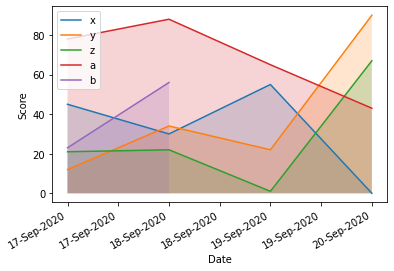
\includegraphics[width=0.7\textwidth,keepaspectratio,angle=270]{5_beamerPPT.png}
\end{frame}

\section{Columns}

\begin{frame}
				\frametitle{Columns}
				
				\begin{columns}
				
					\column{.5\textwidth}
						\blindtext
					\column{.5\textwidth}
						\blindtext

				\end{columns}


\end{frame}

\section{Columns\&Images}

\begin{frame}
	\frametitle{Columns\&Images}
			
				\begin{columns}
				
					\column{.5\textwidth}	
						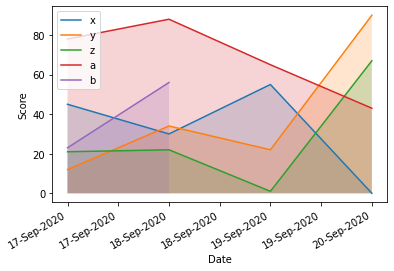
\includegraphics[height=0.5\textheight,keepaspectratio,angle=90]{5_beamerPPT.png}
					
					\column{.5\textwidth}
						\blindtext

				\end{columns}

\end{frame}

\begin{frame}
	\frametitle{Columns\&Images}
			
				\begin{columns}
					
					\column{.5\textwidth}
						\blindtext
				
					\column{.5\textwidth}
					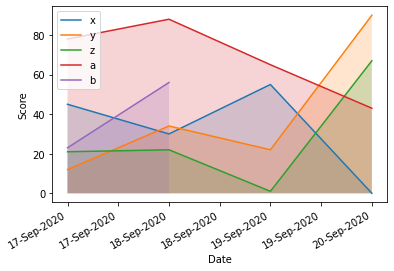
\includegraphics[height=\textwidth,keepaspectratio,angle=270]{5_beamerPPT.png}
				
				\end{columns}

\end{frame}


\end{document}
